\pagestyle{empty}
\section{System Overview\\{\small\tt J.~Mitchard}}

\subsection{Supervisor-Child Architecture}
% another intro to OTP
% what is a SupervisorSupervisor-Child Architecture
% why this is useful
    % gen-servery stuff
The \verb+swarmer+ application has been implemented in a hierarchical process structure using Erlang Supervisor processes\footnote{http://www.erlang.org/doc/man/supervisor.html} that comes as part of the OTP\footnote{http://www.erlang.org/doc/design\_principles/des\_princ.html} \footnote{http://learnyousomeerlang.com/what-is-otp} (Open Telecom Platform). This means that all processes are children of a supervisor process within the applications' supervision tree. Supervisors are responsible for the stopping, starting and restarting of their child processes.
%
\verb+Swarmer+ has one main supervisor, called the \verb+swarm_sup+, this is responsible for the \verb+tile_sup+, \verb+viewer_sup+, \verb+human_sup+, \verb+zombie_sup+, \verb+supplies_sup+ supervisor processes and the \verb+environment+ process.

Apart from \verb+swarm_sup+, all of the supervisors are created with a \verb+simple-one-for-one+ restart strategy, meaning that each of the children will be identical processes using the same code, and should be researted if they crash. \verb+swarm_sup+ is using a \verb+one-for-one+ strategy which can restart it's child processes without affecting the others\footnote{http://www.erlang.org/doc/design\_principles/sup\_princ.html\#id68643}.
% \footnote{http://www.erlang.org/doc/design_principles/sup_princ.html#id68643}.

\begin{figure}[h]
  \centering
  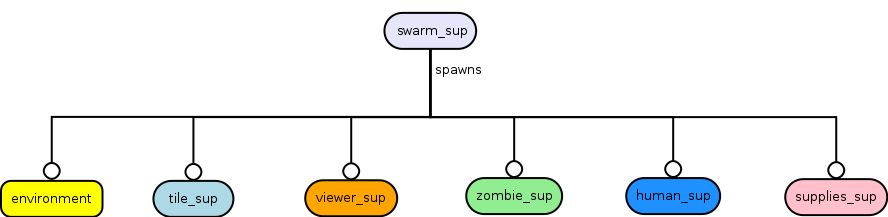
\includegraphics[width=0.8\textwidth]{img/supervisor.png}
\caption{Supervision Tree for Swarmer}
    \label{fig:sup_tree}
\end{figure}

Using an Erlang and OTP application with a process supervision architecture provides a standard set of interface functions, behaviours and more advanced error tracing and reporting functionality.

\subsection{System Architecture}
\label{sys_overview_architecture}
% Overall Architecture
% Link back to evolution and design documents
% Include a new, final Architecture Overview diagram

\subsection{Communication}
% intro to the Communication of processes
% lots of little Communication diagrams
% one overall, simplified one

\clearpage
\endinput
